\begin{frame}{Change of basis}
We have seen how the coordinate vector map $[\hspace{10pt}]_B$ and matrix representations $[T]_B^{B'}$ are two invaluable computational tools for dealing with abstract vector spaces. 
\bpause 
As the notation indicates, both of these operations depend essentially on your \alert{choice of basis or bases}.
This gives rise to the following questions: 
\bb
\ii Given $V$ and two choices of basis, $B$ and $B'$, what is the relation between $[\boldv]_B$ and $[\boldv]_{B'}$?
\ii GIven $T\colon V\rightarrow W$ and two choices of pairs of bases, $(B, B')$ and $(B'', B''')$, what is the relation between $[T]_{B}^{B'}$ and $[T]_{B''}^{B'''}$?
\ee
\pause 
We will tackle both questions in turn. Both answers rely on something called a \alert{change of basis matrix} $\underset{B\rightarrow B'}{P}$. 
\bpause
For question (2), we will look at the slightly less general situation where $T\colon V\rightarrow V$: i.e., the situation where $W=V$, and we choose the same basis for the domain and codomain. I leave the full general case as an exercise. 
\end{frame}
\begin{frame}{Change of basis matrix}
\begin{block}{Theorem/Definition} Given a vector space $V$ of dimension $n$, and two different bases $B$ and $B'$, there is a \alert{unique} $n\times n$ matrix $\underset{B\rightarrow B'}{P}$ satisfying the following defining property:
\[
\underset{B\rightarrow B'}{P}[\boldv]_B=[\boldv]_{B'}.
\]
The matrix $\underset{B\rightarrow B'}{P}$ is called the {\bf change of basis matrix (or transition matrix) from $B$ to $B'$}. 
\end{block}
\bpause
\begin{proof}[Proof/recipe] Let $B=\{\boldv_1,\dots, \boldv_n\}$ and let $B'=\{\boldw_1,\dots,\boldw_n\}$. 

We build $\underset{B\rightarrow B'}{P}$ \alert{column by column}: specifically, $\underset{B\rightarrow B'}{P}$ is the matrix whose $j$-th column is  
\[
\boxed{\boldp_j=[\boldv_j]_{B'}};
\]
i.e., to compute the $j$-th column of $\underset{B\rightarrow B'}{P}$ you must find the $B'$-coordinates of the $j$-th basis element of $B$.  

\pause Thus defined, one can show using the column method that $\underset{B\rightarrow B'}{P}[\boldv_j]_{B}=[\boldv_j]_{B'}$. One then argues that if the condition is true for each basis element $\boldv_j$, then it must be true for all $\boldv$. (Ask your professor for details!) 
\end{proof}
\end{frame}
\begin{frame}
\alert{Example}. For any vector space $V$ and basis $B$, we have $\underset{B\rightarrow B}{P}=I$. 
\bpause
Indeed for any vector $\boldv$, we have $I[\boldv]_B=[\boldv]_B$. Thus $I$ satisfies the defining property of $\underset{B\rightarrow B}{P}$. By uniqueness, it follows that $I=\underset{B\rightarrow B}{P}$ !!
\bpause
\alert{Example}. Let $V=\R^2$. Compute $\underset{B\rightarrow B'}{P}$ where $B=\{\boldv_1=(1,1),\boldv_2=(1,-1)\}$ and $B'=\{(1,2),(2,1)\}$. 

Test that the matrix converts correctly using the vector $\boldv=1(1,1)+3(1,-1)=(4,-2)$. 
\begin{bsolution}
The recipe tells us that 
\begin{eqnarray*}
\underset{B\rightarrow B'}{P}&=&\begin{bmatrix}
\vert &\vert \\
\hspace{7pt}[\boldv_1]_{B'} &\hspace{7pt}[\boldv_2]_{B'}\\
\vert &\vert 
\end{bmatrix}\\
\pause&=&\begin{bmatrix}[rr]1/3&-1\\
1/3&1
\end{bmatrix} \hspace{8pt}\text{(after some computation)}
\end{eqnarray*}
\pause For $\boldv=1(1,1)+3(1,-1)=(4,-2)$, we have $(\boldv)_B=(1,3)$. Thus we should have 
\[
[\boldv]_{B'}=\underset{B\rightarrow B'}{P}[\boldv]_B=\begin{bmatrix}[rr]1/3&-1\\
1/3&1
\end{bmatrix}\begin{bmatrix}
1\\ 3
\end{bmatrix}=\begin{bmatrix}
-8/3\\
10/3 
\end{bmatrix}.
\]
\pause Indeed, one easily verifies that $(4,-2)=-8/3(1,2)+10/3(2,1)$. 
\end{bsolution}

\end{frame}
\begin{frame}{Example}
Take $V=P_2$, $B=\{1,x,x^2\}$ and $B'=\{1,(x-2), (x-2)^2\}$. Compute $\underset{B\rightarrow B'}{P}$. 
\bpause
Follow the recipe: let $\boldp_j$ be the $j$-th column of $\underset{B\rightarrow B'}{P}$. We have (after some computation)
\[
\boldp_1=[1]_{B'}=(1,0,0), \ \boldp_2=[x]_{B'}=(2,1,0), \ \boldp_3=[x^2]_{B'}=(4,4,1).
\]
Thus $\underset{B\rightarrow B'}{P}=\begin{bmatrix}1&2&4\\ 0&1&4\\ 0&0&1  \end{bmatrix}$
\bpause
Let's check with the test vector $p(x)=1+x+x^2$. We have $(p)_B=(1,1,1)$. Thus we should have 
$
[p]_{B'}=\underset{B\rightarrow B'}{P}[p]_B=\begin{bmatrix}1&2&4\\ 0&1&4\\ 0&0&1  \end{bmatrix}\begin{bmatrix}1 \\ 1 \\ 1\end{bmatrix}=\begin{bmatrix}
7\\ 5\\ 1
\end{bmatrix}$.
Equivalently, this means that $p(x)=7+5(x-2)+(x-2)^2$, as one easily verifies. 

\framebreak
\pause\alert{Cool fact}. We could have derived the last equality using the theory of Taylor series. Namely any polynomial can be ``expanded around $x=a$" as 
$
p(x)=\sum_{i=0}^n\frac{p^{(i)}(a)}{a!}(x-a)^i.
$

More generally, this means 
\[
(p(x))_{B'}=(p(a), p'(a), p''(a)/2, \dots , p^{(n)}(a)/n!)
\]
where $B'=\{1,x-a, (x-a)^2,\dots , (x-a)^n\}$. 
\end{frame}
\begin{frame}
\alert{Theorem}. Let $V$ be a vector space of dimension $n$, and let $B$ and $B'$ be two different bases of $V$. 

The change of basis matrix $\underset{B\rightarrow B'}{P}$ is invertible. In fact we have 
\[
(\underset{B\rightarrow B'}{P})^{-1}=\underset{B'\rightarrow B}{P}
\]
\pause
\alert{Proof}. \scriptsize 
I will show that $\underset{B'\rightarrow B}{P}\cdot\underset{B\rightarrow B'}{P}=I_n$, proving that both matrices are invertible, and are in fact the inverses of one another. My proof will only make use of the defining property of change of basis matrices, and their uniqueness.

For any $\boldv$ we compute:
\begin{eqnarray*}
\underset{B'\rightarrow B}{P}\cdot\underset{B\rightarrow B'}{P}[\boldv]_B&=&\underset{B'\rightarrow B}{P}(\underset{B\rightarrow B'}{P}[\boldv]_B)\\
\pause&=&\underset{B'\rightarrow B}{P}[\boldv]_{B'} \hspace{5pt} \text{(prop. of $\underset{B\rightarrow B'}{P}$)}\\
\pause&=&[\boldv]_{B} \hspace{25pt} \text{(prop. of $\underset{B'\rightarrow B}{P}$)}
\end{eqnarray*}
\pause
Thus $\underset{B'\rightarrow B}{P}\cdot\underset{B\rightarrow B'}{P}[\boldv]_B=[\boldv]_B$ for all $\boldv\in V$. But this means $\underset{B'\rightarrow B}{P}\cdot\underset{B\rightarrow B'}{P}$ satisfies the defining property of $\underset{B\rightarrow B}{P}$.  
\bpause
By \alert{uniqueness} of the change of basis matrix, we must have 
\[
\underset{B'\rightarrow B}{P}\cdot\underset{B\rightarrow B'}{P}=\underset{B\rightarrow B}{P}
\]
\pause Lastly, in a previous example we showed that $P_{B\rightarrow B}=I_n$. Thus, 
\[
\underset{B'\rightarrow B}{P}\cdot\underset{B\rightarrow B'}{P}=\underset{B\rightarrow B}{P}=I_n,
\]
as claimed. 

\end{frame}
\begin{frame}{Example: $V=\R^n$ and $B$ is standard}
Consider the simple example where $V=\R^n$, $B$ is the standard basis, and $B'=\{\boldv_1,\dots,\boldv_n\}$ is some nonstandard basis. 
\bspace
I claim the matrix $P=\begin{bmatrix}\vert&\dots &\vert \\ \boldv_1&\cdots&\boldv_n\\ \vert&\dots &\vert \end{bmatrix}$ whose columns are the elements of $B'$ is the change of basis matrix $\underset{B'\rightarrow B} P$. This follows from our recipe since $\boldv_j=[\boldv_j]_B$. (Recall: when $B$ is the standard basis $[(a_1,a_2,\dots, a_n)]_B=(a_1,a_2,\dots, a_n)$ for all $(a_1,a_2,\dots, a_n)\in\R^n$. )
\bpause Since $\underset{B\rightarrow B'}{P}=(\underset{B'\rightarrow B}{P})^{-1}$, we see that in this special case we can compute $\underset{B'\rightarrow B}{P}$ by placing the elements of $B'$ as columns of a matrix, and then compute $\underset{B\rightarrow B'}{P}$ by taking the inverse of this matrix!
\bpause
\alert{Example}. Let $V=\R^2$, $B$ the standard basis for $\R^2$, and $B'=\{(1,\sqrt{3}),(-\sqrt{3},1)\}$. 

%($B'$ was obtained by taking one vector along the line $\ell_{\pi/3}$ and the other vector perpendicular to this. See CW16.) 

Find $P_{B\rightarrow B'}$. 
\begin{bsolution}
The recipe above tells us that $\underset{B'\rightarrow B}{P}=\begin{bmatrix}[rr]1&-\sqrt{3}\\ \sqrt{3}&1 \end{bmatrix}$ and hence that 
\[
\underset{B\rightarrow B'}{P}=(\underset{B'\rightarrow B}{P})^{-1}=\left(\begin{bmatrix}[rr]1&-\sqrt{3}\\ \sqrt{3}&1 \end{bmatrix}\right)^{-1}=\frac{1}{4}\begin{bmatrix}[rr]1&\sqrt{3}\\ -\sqrt{3}&1 \end{bmatrix}.
\]
\end{bsolution}

\end{frame}
\begin{frame}{Alternative technique when $V=\R^n$}
The following is another technique for computing $\underset{B\rightarrow B'}{P}$ in the \alert{special case} where $V=\R^n$. 
\bpause 
\alert{1.} Let $\widetilde{B}$ and $\widetilde{B'}$ be the matrices obtained by arranging the elements of $B$, respectively $B'$, as columns of a matirx.  Build the augmented matrix
\[
\begin{bmatrix}[c|c]
\widetilde{B'}& \widetilde{B}
\end{bmatrix} 
\]
\bpause
\alert{2.} Row reduce the augmented matrix until the left hand side is $I_n$:
\[
\begin{bmatrix}[c|c]
I_n& Q
\end{bmatrix} 
\]
Then $Q=\underset{B\rightarrow B'}{P}$. 
\bpause
Why does this work? 
\bpause The row reduction process amounts to multiplying both matrices on the left by $(\widetilde{B'})^{-1}$: that is, the matrix $Q$ is $(\widetilde{B'})^{-1}\widetilde{B}$. As we saw in the last example, however, letting $S$ be the \alert{standard basis} of $\R^n$, we have 
\[
(\widetilde{B'})^{-1}=\underset{S\rightarrow B'}{P} \text{ and } \widetilde{B}=\underset{B\rightarrow S}{P}
\]
Thus $Q=\underset{S \rightarrow B'}{P}\cdot \underset{B\rightarrow S}{P}=\underset{B\rightarrow B'}{P}$. (This last equality follows from one of the exercises.) 
\end{frame}
\begin{frame}{Change of basis for transformations}
We now investigate how our choice of basis affects matrix representations of linear transformations. As mentioned above, we only consider the special case where $T\colon V\rightarrow V$ and we are comparing matrix representations $[T]_B$ and $[T]_{B'}$ for two choices of basis for $V$. 
\pause
\begin{theorem}[Change of basis for transformations]
\label{Th:changeofbasis}
Let $V$ be finite-dimensional, let $T\colon V\rightarrow V$ be linear, and let $B$ and $B'$ be two bases for $V$.
\pause Then 
\begin{align}
[T]_{B'}&=\underset{B\rightarrow B'}{P}[T]_B\underset{B'\rightarrow B}{P}\\
&=\left( \underset{B'\rightarrow B}{P}\right)^{-1}[T]_B\underset{B'\rightarrow B}{P}
\end{align}
\end{theorem}

\end{frame}
\begin{frame}{Pro-tip}
 It is easy to get the various details of the change of basis formula wrong. Here is how I organize things in my mind. 
 \bb
 \pause
 \ii We wish to relate $[T]_{B'}$ and $[T]_B$ with an equation of the form $[T]_{B'}=*[T]_B*$, where the asterisks are to be replaced with change of basis matrices or their inverses. Think of the three matrices on the RHS as a sequence of three things done to coordinate vectors, reading from right to left. 
\pause \ii $[T]_{B'}$ takes as inputs $B'$-coordinates of vectors, and outputs $B'$-coordinates. Thus the same should be true for $*[T]_B*$. 
 \pause \ii Since $[T]_B$ takes as inputs $B$-coordinates, we must \alert{first} convert from $B'$-coordinates to $B$-coordinates. So we should have $[T]_{B'}=*[T]_B\underset{B'\rightarrow B}{P}$. 
 \pause \ii Since $[T]_B$ outputs $B$-coordinates, we need to then convert back to $B'$-coordinates. Thus $[T]_{B'}=\underset{B\rightarrow B'}{P}[T]_B\underset{B'\rightarrow B}{P}$. 
 \pause\ii If desired you may replace $\underset{B\rightarrow B'}{P}$ with $\left( \underset{B'\rightarrow B}{P}\right)^{-1}$. 
 \ee
\end{frame}
\begin{frame}{Proof of change of basis theorem}
  
 {\scriptsize
\alert{Theorem recap}. Let $V$ be finite-dimensional, let $T\colon V\rightarrow V$ be linear, let $B$ and $B'$ be two bases for $V$, and let $A=[T]_B$, $A'=[T]_{B'}$. 
\bspace
Then 
$\boxed{A=(\underset{B\rightarrow B'}{P})^{-1}A'\underset{B\rightarrow B'}{P}}$
and 
$\boxed{A'=(\underset{B'\rightarrow B}{P})^{-1}A\underset{B'\rightarrow B}{P}}$
}

\bpause
First recall that $\underset{B'\rightarrow B}{P}=(\underset{B\rightarrow B'}{P})^{-1}$. Using this fact, it is easy to see that the second equality follows from the first by multiplying on the left and right by an appropriate matrix and its inverse. 
\bpause 
We prove the first equality using the \alert{uniqueness property} of $A=[T]_B$. 
\bpause
That is, set $C=(\underset{B\rightarrow B'}{P})^{-1}A'\underset{B\rightarrow B'}{P}$. 

To show $C=A$, we need only show $[T(\boldv)]_B=C[\boldv]_B$ for all $\boldv\in V$. Here goes:
\pause
\begin{eqnarray*}
C[\boldv]_B&=&(\underset{B\rightarrow B'}{P})^{-1}A'\underset{B\rightarrow B'}{P}[\boldv]_B \\
\pause &=&\underset{B'\rightarrow B}{P}A'\underset{B\rightarrow B'}{P}[\boldv]_B\hspace{10pt} (\text{since }\underset{B'\rightarrow B}{P}=(\underset{B\rightarrow B'}{P})^{-1})\\
\pause &=&\underset{B'\rightarrow B}{P}A'[\boldv]_{B'} \hspace{10pt} \text{(prop. of $\underset{B\rightarrow B'}{P}$)}\\
\pause &=&\underset{B'\rightarrow B}{P}[T(\boldv)]_{B'} \hspace{10pt} \text{(prop. of $A'=[T]_{B'}$)}\\
\pause&=&[T(\boldv)]_{B}
\end{eqnarray*}
\pause Amazing! We didn't even have to get our hands dirty. 
\end{frame}
\begin{frame}{Example}
 Let $T\colon P_2\rightarrow P_2$ be defined as $T(p(x))=p(x)+2p'(x)+xp''(x)$. 
 \bb
 \ii Let $B=\{1, x, x^2\}$. Compute $[T]_B$. 
 \ii Let $B'=\{1+x+x^2, 1+x, 1+x^2\}$. Use the change of basis formula to compute $[T]_{B'}$. 
 \ee
 \pause
 We easily compute $[T]_B=\begin{bmatrix}
 1&2&0\\
 0&1&4\\
 0&0&1
 \end{bmatrix}
 $
 using our usual recipe. 
 \bpause We can also easily compute $\underset{B'\rightarrow B}{P}=\begin{bmatrix}
 1&1&1\\
 1&1&0\\
 1&0&1
 \end{bmatrix}$, essentially by inspection. 
 
 (In general it is easy to compute the change of basis matrix from a nonstandard basis to the standard basis.) 
 \bpause
 It follows that 
 \begin{align*}
 [T]_B'&=\underset{B\rightarrow B'}{P}[T]_B\underset{B'\rightarrow B}{P}=\left( \underset{B'\rightarrow B}{P}\right)^{-1}[T]_B\underset{B'\rightarrow B}{P}\\
 &=\left( \begin{bmatrix}
 1&1&1\\
 1&1&0\\
 1&0&1
 \end{bmatrix}\right)^{-1}\begin{bmatrix}
 1&2&0\\
 0&1&4\\
 0&0&1
 \end{bmatrix}
\begin{bmatrix}
 1&1&1\\
 1&1&0\\
 1&0&1
 \end{bmatrix}=
 \begin{bmatrix}[rrr]
 3&-2&4\\
 2&3&0\\
 -2&2&-3
 \end{bmatrix}
 \end{align*}
\end{frame}
\begin{frame}
 The change of basis formula is often used in the following type of situation. 
\bb
\ii I am interested in a linear transformation $T\colon V\rightarrow V$, where $V$ is finite-dimensional. 
\pause \ii I would like to compute $A=[T]_B$ with respect to a specific basis $B$. (Maybe $B$ is a standard basis for $V$ that I prefer to use.) 
\pause \ii For whatever reason, it is easier to compute $A'=[T]_{B'}$ with respect to some other basis $B'$
\pause \ii Thus we first compute $[T]_{B'}$, then compute $[T]_B$ via the formula 
\[
[T]_B=\underset{B'\rightarrow B}{P}[T]_B'\underset{B\rightarrow B'}{P}.
\]
\ee
The next example nicely illustrates this. 
\end{frame}
\begin{frame}{Example: orthogonal projection revisited}
Let $T\colon \R^3\rightarrow\R^3$ be orthogonal projection onto the plane $\mathcal{P}: x+y+z=0$, as defined earlier. We would like to derive a formula for $T$, which amounts to finding the $A$ such that $T=T_A$. 
\bpause 
As previously observed we have $A=[T]_B$, where $B$ is the \alert{standard basis} for $\R^3$. We can compute $[T]_B$ by first computing $[T]_{B'}$ for a cleverly chosen \alert{nonstandard} basis $B'$, and then using the change of basis formula. 
\bpause 
As done previously, we let $B'=\{(1,-1,0), (1,0,-1), (1,1,1)$. Since $T$ maps the first two vectors to themselves, and the third vector to $(0,0,0)$, we have $[T]_{B'}=\begin{bmatrix}
1&0&0\\
0&1&0\\
0&0&0
\end{bmatrix}$. (Go back to original example for details.) 
\bpause 
Then 
\begin{align*}
A&=[T]_B=\underset{B'\rightarrow B}{P}[T]_{B'}\underset{B\rightarrow B'}{P}\\
&=\begin{bmatrix}[rrr]
1&1&1\\
-1&0&1\\
0&-1&1
\end{bmatrix}
\begin{bmatrix}
1&0&0\\
0&1&0\\
0&0&0
\end{bmatrix}
\left( \begin{bmatrix}[rrr]
1&1&1\\
-1&0&1\\
0&-1&1
\end{bmatrix}\right)^{-1}
=\frac{1}{3}\begin{bmatrix}[rrr]
2&-1&-1\\
-1&2&-1\\
-1&-1&2
\end{bmatrix}
\end{align*}
\pause
Lo and behold, we have rediscovered our matrix formula for orthogonal projection onto $\mathcal{P}$!! 

(Note: since $B$ is the standard basis in this case, $\underset{B'\rightarrow B}{P}$ was easy to compute. )
\end{frame}
\begin{frame}{Similar matrices}
Let $A=[T]_B$ and $A'=[T]_{B'}$ be two different representations of $T\colon V\rightarrow V$, and set $P=\underset{B'\rightarrow B}{P}$. Then we have $A'=P^{-1}AP$, according to the change of basis formula for transformations.  We say $A$ and $A'$ are \alert{similar matrices} in this case. 
\pause
\begin{definition}
Matrices $A, A'\in M_{nn}$ are {\bf similar} if there is an invertible matrix $P$ such that $A'=P^{-1}AP$. 
\end{definition} 
\bpause
This notion of similarity is a technical one, but the name is fitting: $A$ and $A'$ really are similar in the sense that they are just two different matrix representations of the same linear transformation! (See Holy Commutative Tent of Linear Algebra on next slide.) 
\bpause 
As we will see in coming sections, matrices that are similar in this technical sense do indeed share many of the same properties. We now have the theoretical foundation to understand why this is so: they simply inherit these common properties from the overlying linear transformation $T$, of which they are but earthly shadows. 
\bpause
There is but one true $T$!
\end{frame}
\begin{frame}
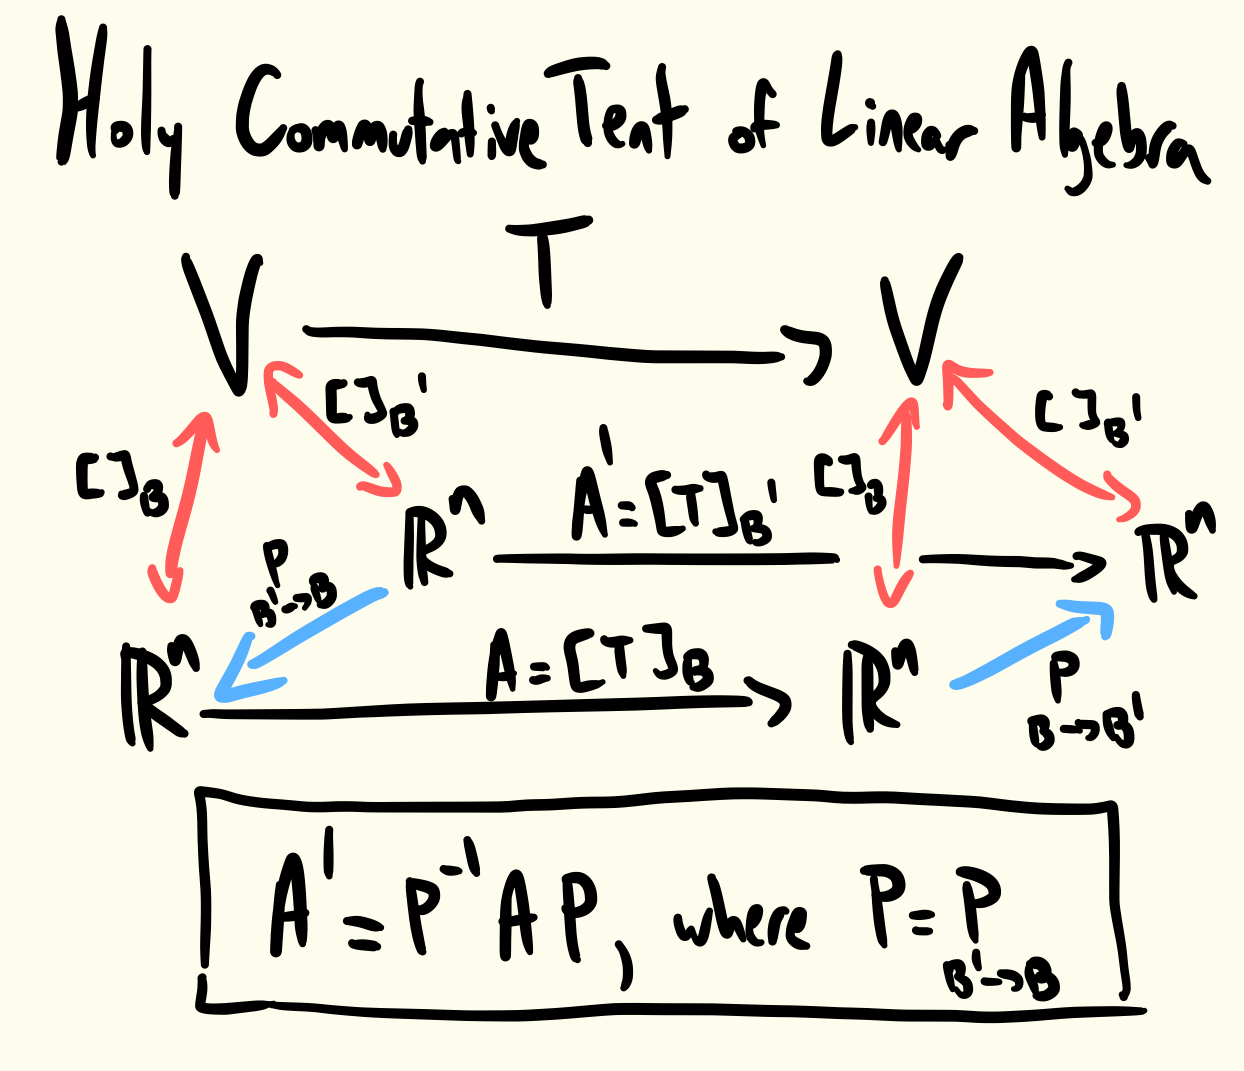
\includegraphics[width=4in]{Images/HolyCommutativeTent}

\end{frame}
